\documentclass[10pt, aspectratio=1610, natbib, handout]{beamer}
\usepackage{common}

\title[GE with Prices]{
  \textbf{General Equilibrium in Representative- and Heterogeneous-Agents Models with Explicit Prices}
}

\subtitle[Macro 3: TA\#4]{
  \textbf{Macroeconomics 3:} TA class \#4
}

\author[A.~Pasqualini]{
  Andrea Pasqualini
}

\institute[Bocconi]{Bocconi University}

\date{
  1 March 2021
}

\begin{document}

  \begin{frame}
    \maketitle
  \end{frame}

  \begin{frame}
    \frametitle{Plan for Today}

    Objective: \textbf{Solve for the equilibrium when explicit prices are involved}

    \vfill\pause

    Two (sub-) goals:
    \begin{itemize}
      \item Learn how to solve GE macro models when prices are involved
      \item Learn how to solve GE macro models when agents are heterogeneous
    \end{itemize}

  \end{frame}

  \begin{frame}
    \frametitle{Working Example}

    Consider this simple exchange economy with exogenous endowments
    \begin{align*}
      \max_{C_t, A_{t+1}} &\; \E_0 \left( \sum_{t=0}^{\infty} \beta^t \frac{C_t^{1-\gamma}}{1-\gamma} \right) \\
      \text{s.t.} &\;
      \begin{cases}
        C_t + A_{t+1} \leq \alert{Y_t} + (1 + \alert{r}_t) A_t \\
        A_{t+1} \geq \underline{A}
      \end{cases}
    \end{align*}

    \vfill\pause

    Today we look at two versions:
    \begin{itemize}
      \item $Y_t = Y$ deterministically \hfill\dimmer{(representative-agent economy)}
      \item $Y_t$ is stochastic and idiosyncratic \hfill\dimmer{(heterogeneous-agents economy)}
    \end{itemize}

    \vfill\pause

    When $Y_t$ is stochastic, we assume $Y_t \in \{ Y^l, Y^h \}$, with
    \begin{equation*}
      P(Y_{t+1} | Y_t) = \Pi =
      \begin{bmatrix}
        \pi & 1 - \pi \\
        1 - \pi & \pi
      \end{bmatrix}
    \end{equation*}

  \end{frame}

  \begin{frame}
    \frametitle{RA Economy: Market Clearing}

    The model is numerically uninteresting, the closed form solution for the price $r$ is given by imposing $A_t^* = 0$ for all periods $t$, because we have one representative agent, therefore the net financial position must be zero
    \begin{equation*}
      \begin{cases}
        r_t^* = 1 / \beta - 1 & \forall\ t \\
        C_t^* = Y & \forall\ t \\
        A_t^* = 0 & \forall\ t
      \end{cases}
    \end{equation*}

    \vfill\pause

    The Bellman equation
    \begin{align*}
      V(A) = \max_{C, A'} &\; \frac{C^{1-\gamma}}{1-\gamma} + \beta\ V(A') \\
      \text{s.t.} &\;
      \begin{cases}
        C + A' \leq Y + (1 + r) A \\
        A' \geq \underline{A}
      \end{cases}
    \end{align*}

    \vfill\pause

    The market clearing condition $A_t^* = 0$ translates into this condition on the policy function: $A'(0) = 0$
    \begin{itemize}
      \item If $A'(0) > 0$, excess demand: RA wants to save, but nobody is there to sell assets
      \item If $A'(0) < 0$, excess supply: RA wants to borrow, but nobody is there to buy assets
    \end{itemize}

  \end{frame}

  \begin{frame}
    \frametitle{RA Economy: Strategy for Numerical Solution}

    New element relative to past TA classes: price $r$
    \begin{itemize}
      \item Solve VFI/PFI given a numerical a value for $r$
      \item Check market clearing condition for asset holdings
        \begin{itemize}
          \item If net excess demand \textgreater\ 0 (i.e., excess demand), $r$ was too low: do it all again with higher $r$
          \item If net excess demand \textless\ 0 (i.e., excess supply), $r$ was too high: do it all again with lower $r$
          \item If there is zero excess supply/demand, $r$ was just right: model solved!
        \end{itemize}
    \end{itemize}

    \vfill\pause

    The net excess demand in this context is exactly $A'(0)$

    \vfill\pause

    \dimmer{You can see why VFI/PFI must be fast: need to solve for policy functions over and over again}

  \end{frame}

  \begin{frame}
    \frametitle{RA Economy: Intuition on Why/How This Works}

    \begin{columns}[T]
      \begin{column}{0.5\textwidth}
        \begin{itemize}
          \item Net excess demand: $Z(r) \equiv D(r) - S(r)$
          \item From theory, $Z(r)$ is decreasing
          \item From theory, $\exists\ r^*: Z(r^*) = 0$
        \end{itemize}
      \end{column}
      \begin{column}{0.4\textwidth}
        \textbf{Algorithm:} Given a guess $r^{(j)}$
        \begin{itemize}
          \item if $Z \left( r^{(j)} \right) > 0$, then $r^{(j)} < r^*$
          \item if $Z \left( r^{(j)} \right) < 0$, then $r^{(j)} > r^*$
          \item Set $r^{(j+1)}$ accordingly and repeat
        \end{itemize}
      \end{column}
    \end{columns}

    \vfill\pause

    \begin{figure}
      \centering
      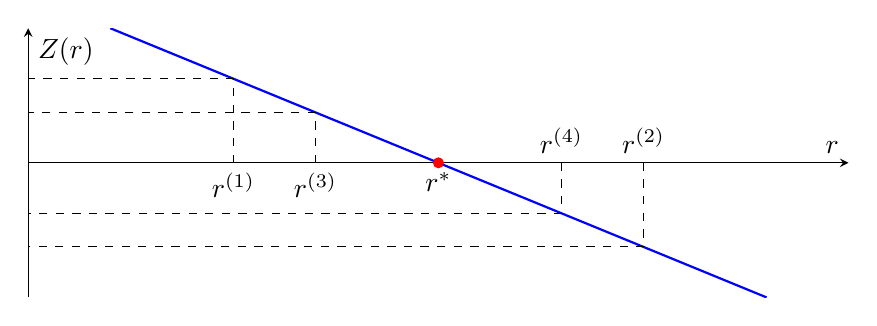
\begin{tikzpicture}
        \begin{axis}[footnotesize, xmin=0, xmax=5, enlarge x limits={1}, width=12cm, height=5cm, ticks=none, axis lines=middle, xlabel={$r$}, ylabel={$Z(r)$}]
          \addplot[domain=0.5:4.5, thick, color=blue, samples=3]{2.5 - x};
          \draw[black, dashed] (1.25, 0) -- (1.25,  1.25) -- (0,  1.25);  % r1
          \draw[black, dashed] (3.75, 0) -- (3.75, -1.25) -- (0, -1.25);  % r2
          \draw[black, dashed] (1.75, 0) -- (1.75,  0.75) -- (0,  0.75);  % r3
          \draw[black, dashed] (3.25, 0) -- (3.25, -0.75) -- (0, -0.75);  % r4
          \fill[red]{(2.5, 0) circle (2pt)};
          \node[below] at (2.5, 0) {$r^*$};
          \node[below] at (1.25, 0) {$r^{(1)}$};
          \node[above] at (3.75, 0) {$r^{(2)}$};
          \node[below] at (1.75, 0) {$r^{(3)}$};
          \node[above] at (3.25, 0) {$r^{(4)}$};
          \node[left] at (0,  1.25) {$Z(r^{(1)})$};
          \node[left] at (0, -1.25) {$Z(r^{(3)})$};
          \node[left] at (0,  0.75) {$Z(r^{(4)})$};
          \node[left] at (0, -0.75) {$Z(r^{(2)})$};
        \end{axis}
      \end{tikzpicture}
    \end{figure}

  \end{frame}

  \begin{frame}
    \frametitle{RA Economy: Coding Approach}

    \textbf{Objective:} write a function that takes a price and returns the net excess demand at that price \\
    \textbf{Objective:} use a zero-finding routine that finds the zero of the aforementioned function

    \vfill\pause

    The function $Z(r)$, given calibrated parameters and relevant grids
    \begin{enumerate}
      \item Solves VFI/PFI and extracts the policy functions
      \item Computes the net excess demand
      \item Returns the numerical value of the net excess demand
    \end{enumerate}

    \vfill\pause

    Then, use any of the appropriate functions in \texttt{scipy.optimize}:
    \begin{itemize}
      \item \texttt{bisect}
      \item \texttt{brentq}
      \item \texttt{ridder}
      \item \texttt{toms748}
    \end{itemize}

    \vfill

    Learn more at \url{https://docs.scipy.org/doc/scipy/reference/optimize.html}

  \end{frame}

  \begin{frame}
    \frametitle{HA Economy: Market Clearing}

    \begin{columns}[T]
      \begin{column}{0.48\textwidth}
        The Bellman equation
        \begin{align*}
          V(A, Y) = \max_{C, A'} &\; \frac{C^{1-\gamma}}{1-\gamma} + \beta\ \E \left( V(A', Y') \middle| A, Y \right) \\
          \text{s.t.} &\;
          \begin{cases}
            C + A' \leq Y + (1 + r) A \\
            A' \geq \underline{A} \\
            P(Y' | Y) = \Pi
          \end{cases}
        \end{align*}
      \end{column}
      \begin{column}{0.48\textwidth}
        We have
        \begin{itemize}
          \item An exogenous Markov chain $P(Y' | Y)$
          \item A policy function $A'(A, Y)$
        \end{itemize}
        \vspace{1em}
        We obtain
        \begin{itemize}
          \item An endogenous distribution $\lambda_t(A, Y)$
          \item An ergodic endogenous distr.~$\lambda(A, Y)$
        \end{itemize}
      \end{column}
    \end{columns}

    \vfill\pause

    Market clearing: total savings = total borrowings
    \begin{equation*}
      \int_A \int_Y \lambda(A, Y)\ A'(A, Y)\ \text{d} Y\ \text{d} A = 0
    \end{equation*}
    \begin{itemize}
      \item For the household, $r$ is taken as given (like a parameter)
      \item For the equilibrium, $r$ depends on the infinite-dimensional object $\lambda(A, Y)$
      \item We say that $\lambda(A, Y)$ is an infinite-dimensional state variable (for the equilibrium!): infeasible in a computer, must approximate
    \end{itemize}

    \vfill\pause

    \textbf{Objective:} approximate the ergodic endogenous distribution $\lambda(A, Y)$
  \end{frame}

  \begin{frame}
    \frametitle{HA Economy: The Endogenous Distribution of Agents}

    \begin{itemize}
      \item The exogenous matrix $\Pi$ maps $Y$ into $Y'$
      \item The endogenous policy function $A'(A, Y)$ maps $(A, Y)$ into $A'$
      \item Combine them to map $(A, Y)$ into $(A', Y')$
    \end{itemize}

    \vfill\pause

    Formally, let $\lambda_t(A, Y)$ be the endogenous joint distribution of agents at period $t$
    \begin{equation*}
      \lambda_{t+1}(A', Y') = P(Y' | Y) \cdot A'(A, Y) \cdot \lambda_t(A, Y)
    \end{equation*}

    \vfill\pause

    \begin{itemize}
      \item The transition from $(A, Y)$ to $(A', Y')$ is regulated by an endogenous Markov process
      \item The distribution $\lambda(A, Y)$ is the ergodic distribution associated to such Markov process
      \item We normally focus on \textbf{ergodic recursive equilibria} \hfill\dimmer{(else, too much going on)}
    \end{itemize}

  \end{frame}

  \begin{frame}
    \frametitle{HA Economy: Strategy for Numerical Solution}

    \begin{itemize}
      \item Solve VFI/PFI given a numerical value for $r$
      \item Recode the policy function as a set of transition matrices ${(\bar{A}^k)}_{k=0}^{m}$ such that
        \begin{equation*}
          \bar{A}^k_{[i, j]} \equiv
          \begin{cases}
            1 & \text{ if } A'(A_i, Y_k) = A_j \\
            0 & \text{ if } A'(A_i, Y_k) \neq A_j
          \end{cases}
        \end{equation*}
      \item Combine the matrices ${(\bar{A}^k)}_{k=0}^{m}$ in a block diagonal matrix such that
        \begin{equation*}
          \underset{[n m \times n m]}{\bar{A}} \equiv
          \begin{bmatrix}
            \bar{A}^1 & 0 & \cdots & 0 \\
            0 & \bar{A}^2 & \cdots & 0 \\
            \vdots & \vdots & \ddots & \vdots \\
            0 & 0 & \cdots & \bar{A}^{m}
          \end{bmatrix}
        \end{equation*}
      \item Compute the endogenous transition matrix Q as \hfill\dimmer{(maps $(A, Y)$ into $(A', Y')$)}
        \begin{equation*}
          \underset{[n m \times n m]}{Q} \equiv (\Pi \otimes I_n) \cdot \bar{A}
        \end{equation*}
      \item Compute the ergodic distribution associated with the transition matrix $Q$: that is $\lambda(A, Y)$
    \end{itemize}

  \end{frame}

  \begin{frame}
    \frametitle{HA Economy: Coding Approach}

    \textbf{Objective:} write a function that takes a price and returns the net excess demand at that price \\
    \textbf{Objective:} use a zero-finding routine that finds the zero of the aforementioned function

    \vfill\pause

    The function $Z(r)$, given calibrated parameters and relevant grids
    \begin{enumerate}
      \item Solves VFI/PFI and extracts the policy functions
      \item \alert{Constructs the ergodic distribution of agents}
      \item Computes the net excess demand
      \item Returns the numerical value of the net excess demand
    \end{enumerate}

    \vfill\pause

    Then, use any of the appropriate functions in \texttt{scipy.optimize}:
    \begin{itemize}
      \item \texttt{bisect}
      \item \texttt{brentq}
      \item \texttt{ridder}
      \item \texttt{toms748}
    \end{itemize}

    \vfill

    Learn more at \url{https://docs.scipy.org/doc/scipy/reference/optimize.html}

  \end{frame}

  \begin{frame}
    \frametitle{Practice Time}

    Moving to a Jupyter Notebook

  \end{frame}

  \begin{frame}
    \frametitle{Exercises}

    \begin{enumerate}
      \item Use the code I have showed for both examples
        \begin{enumerate}
          \item Replace VFI with PFI
          \item Report on the speed improvements
        \end{enumerate}
      \vfill
      \item The second example we saw today is essentially the Huggett model
        \begin{enumerate}
          \item Adapt the code such that it is written as one coherent Python \texttt{class}
          \item Generalize the code to accept any AR(1) process for the endowment process
          \item In what sense the transition matrix $Q$ is obtained the quick-and-dirty way? How could you address the issue?
        \end{enumerate}
    \end{enumerate}

  \end{frame}

\end{document}
